% 来源：OEBPS/Text/Section0001_split_002.xhtml#sigil_toc_id_18

\BookChapter{9}
\section[第9章\q 投资营销谎言4：“我是你的经纪人，我是来帮你的”]{第9章\\ 投资营销谎言4：“我是你的经纪人，我是来帮你的”}

\begin{BookQuote}
有的事情，你就是很难让一个人弄明白，因为他赚这份工资靠的就是你不明白这件事情。

\hfill ——厄普顿·辛克莱
\end{BookQuote}

\subsection{开门见山}

现在让我们回顾一下。

那些兜售给我的公募基金，向我收取的费用简直是天价，拿走了我未来养老金潜在投资收益的70\%。

在一段持续较长的时间里，96\%的主动管理型公募基金的业绩跑输了市场，或者它们的业绩基准。

我买一只指数基金，“成为”市场或者模拟市场，其投资成本很低。购买主动管理型公募基金的成本要比指数基金高上10\textasciitilde{}30倍。

公募基金在市场营销广告上所宣传的投资业绩往往高于投资者实际上得到的投资业绩，因为它们在广告上说的是时间加权投资收益，不是资金加权投资收益。资金加权投资收益才是我们真正拿到手的投资收益，而时间加权投资收益是基金经理用来做广告的，它看起来很美，实际上得不到。

就像电影的大结局一样，你的理财经理会深情地凝望着你的双眼，告诉你，他会把你的最高利益放在心上。这很有可能是真的，他发自内心地相信，他是在帮你。他根本不明白，或者他从来没有受过这方面的教育。天哪，他给你的是这样的投资建议，他是这么说的，可能他个人的投资理财也是这么做的。

\subsection{呼哧！呼哧！}

绝大多数美国人买了公募基金，相当于受了千刀万剐的死刑，却没有多少人能醒悟过来，奋起反抗。怎么可能有这样的事情呢？答案是他们已经受到蒙蔽好几十年了，都习惯了。我把这些真相讲出来，大多数人听了都非常怀疑金融服务行业从业者的良知，怀疑他们说自己的愿望是“帮助”客户取得投资成功。但是互相矛盾的信息每天如滔滔江水一般涌来，市场营销持续不断地狂轰滥炸，投资者很快就要崩溃了，更不用说提高日常生活水平了。很多人烦透了，干脆把自己的金融事务变成了自动驾驶模式。他们投降了，成为逆来顺受的客户羊群中的一员。“希望”成了他们采取的策略。

你知道自己并不孤独，从社交情感上会让你感觉很舒服。这让我想起我在探索频道看到的一集野生动物节目，那些羚羊小心翼翼地接近鳄鱼密集的水域，只为了喝上几口水，尽管就在几分钟之前，鳄鱼的大嘴刚咬住它的同伴，把它拖下了水！这些动物是不是太愚蠢了？不！这些动物知道，不喝水自己就有可能渴死，因为非洲的太阳太毒了，所以它们在精心算计之后还是选择了冒险。我们很多人之所以买公募基金，也是出于同样的想法。我们知道我们不能坐在河岸边缘，因为通货膨胀会毁掉我们的财富，如果我们只是拿着现金不动，长期来看，货币就会大幅贬值。所以，和邻居们还有同事们一起，我们尽管十分恐惧和害怕，但还是从河岸走到河边，这样做至少还有一点希望：呼哧！呼哧！喝上两口水。

黑色星期一，网络股泡沫，2008年金融危机。

一直以来，我们把自己家庭未来的生活品质完全托付给证券公司和银行，它们却什么风险也不承担，一年接一年地刷新酬金纪录。

2014年年初，我在写本书的时候，美国股市还在继续上涨。2009—2013年年底，美国股市上涨了131\%（包括红利再投资）。这是美国历史上第五大牛市。投资者看着自己的投资账户余额不断上涨，再次感觉非常舒服。基金经理们和高管们也在大把大把地捞钱。但是鳄鱼也在大口吃进。

\subsection{如何保护投资人？}

2009年下半年，参议员巴尼·弗兰克和克里斯·多德提出了一份立法建议，它被称为《多德–弗兰克华尔街改革和消费者权益保护法案》。一年之后，在金融服务业人员的密集游说之后，另一个版本的法案通过了，但是其严厉程度比最初的版本低多了。没有人停止问这个非常明显的问题：如何保护投资人？

我们可以信任谁来管理我们的财务未来呢？是那些卖给我们收费昂贵的公募基金的理财经理和股票经纪人吗？是那些基金经理，玩着合法但是见不得人的不正当游戏的家伙吗？是那些高频交易员，抢在客户下单之前提前交易，通过大量快速高频交易赚到百万美元的人吗？就在最近两三年，我们看到了有些流氓交易员给银行造成了几十亿的损失。而且大的证券公司，比如全球曼氏金融挪用客户资金，最终宣告破产；全球最大的对冲基金之一，内部人承认内幕交易；银行的交易员被指控操纵LIBOR（伦敦同业拆借利率）——全球最广泛使用的短期利率基准。

\begin{figure}[htbp]
\centering
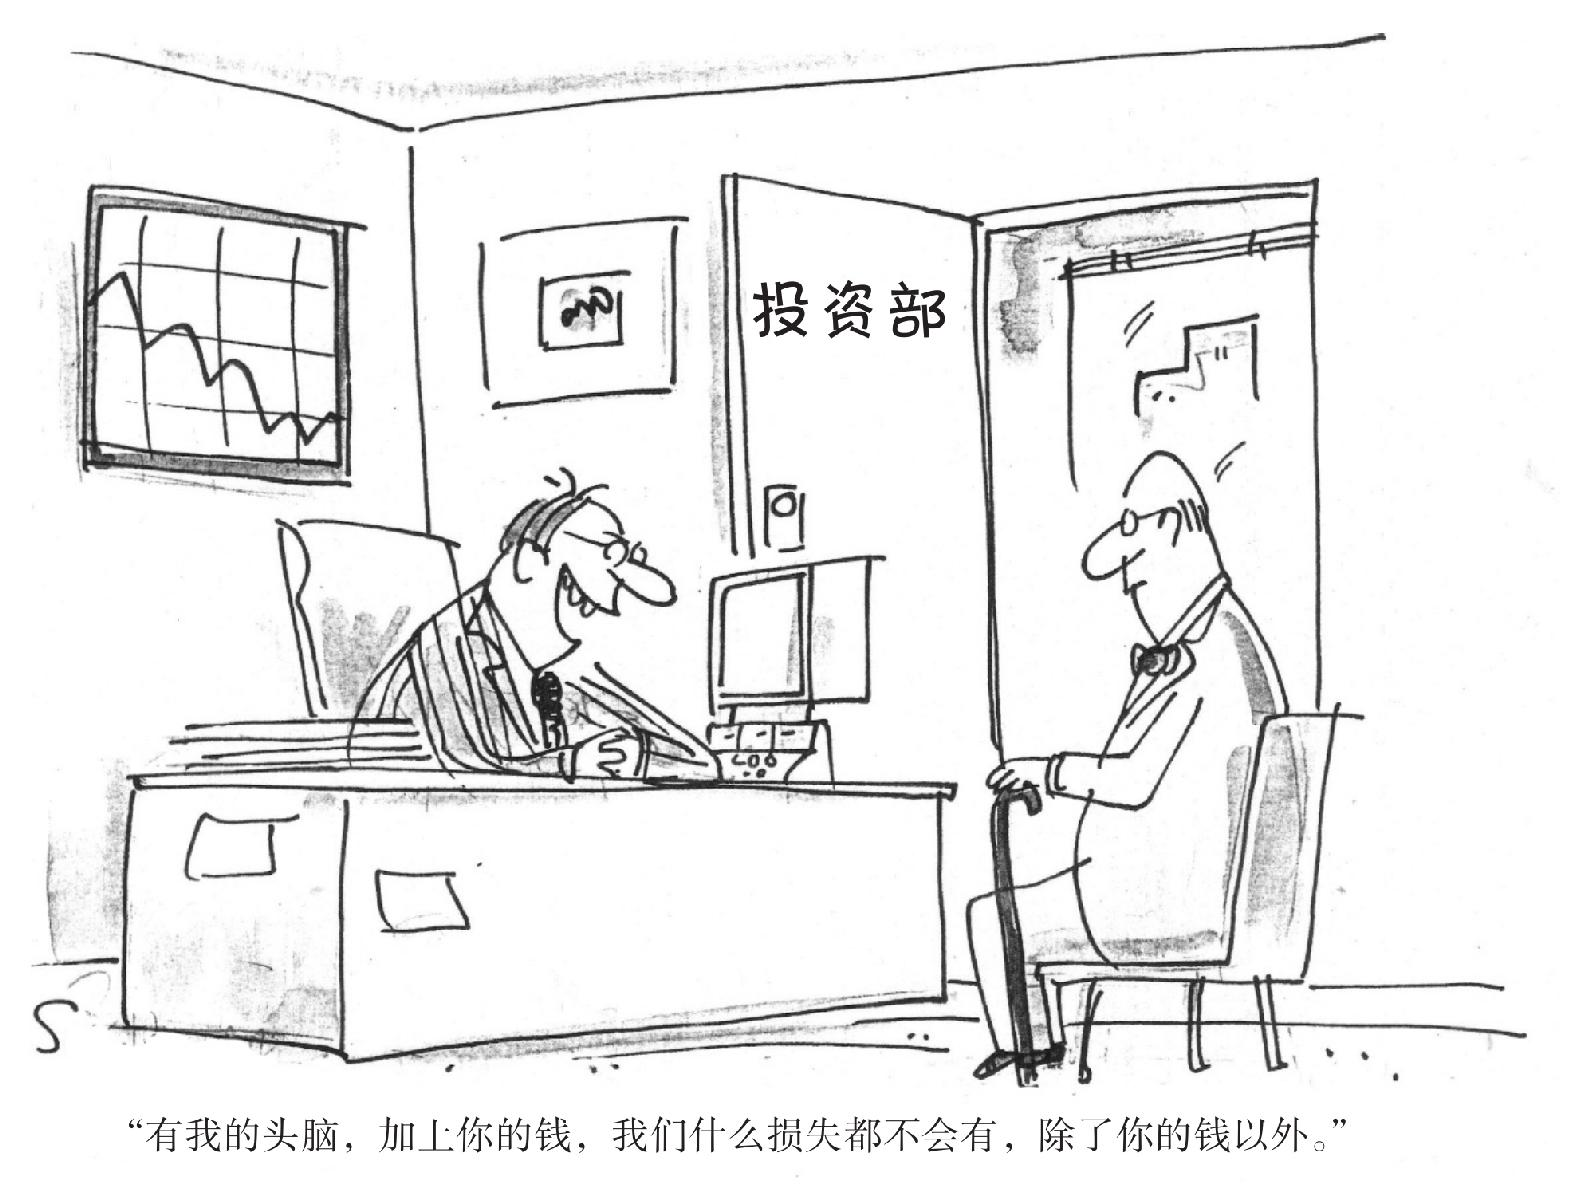
\includegraphics[width=0.78\linewidth,keepaspectratio]{image/9-1.jpg}
\caption{}\label{fig:9-1}
\end{figure}

\subsection{大厨不吃自己做的饭}

那些不断地向我们推销产品，持续对我们施加影响的人，都是些心口不一的家伙。他们说一套，做一套。2009年，晨星基金公司发布的一份研究报告，如同给人打了一针清醒剂，公司有关人员追踪了4300多只主动管理型公募基金，结果发现，49\%的基金经理没有持有一份自己管理的基金。是的，那些大厨自己做的饭，他们自己并不吃。

其余51\%的基金经理尽管持有自己管理的基金，但是跟他们自己拿到的薪酬和个人财富相比，这部分基金简直是九牛一毛。要知道，这些人都是靠投资技能拿到了百万年薪的，有的时候甚至是千万年薪。

\begin{itemize}
\item 2126名基金经理持有自己管理的基金金额为零。
\item 159名基金经理持有自己管理的基金金额为1\textasciitilde{}1万美元。
\item 390名基金经理持有自己管理的基金金额为1万\textasciitilde{}5万美元。
\item 285名基金经理持有自己管理的基金金额为5万\textasciitilde{}10万美元。
\item 679名基金经理持有自己管理的基金金额为10万\textasciitilde{}50万美元。
\item 197名基金经理持有自己管理的基金金额为50万\textasciitilde{}100万美元。
\item 413名基金经理持有自己管理的基金金额为超过100万美元。
\end{itemize}

一个明显的问题是，如果这些管理基金的人都不投资他们自己管理的基金，那么为什么我们要投资？好问题！

大厨不吃自己做的饭菜，是因为里面有些原料很不好，或者他知道厨房到底是什么样子，闻起来是什么味道。这些基金经理一点儿也不傻——他们对幕后的事情门儿清。

\subsection{客户的游艇在哪里？}

小弗莱德·施韦德是一名职业交易员，在1929年的股市大崩盘里亏了很多钱，从此退出华尔街。1940年他写了一本书《客户的游艇在哪里？》，这本书成了一本投资经典名著。这个书名来源于一个笑话，过去讲了很多年，有各种各样的版本，但是按照施韦德本人的版本是这样讲述的：有个成功的华尔街证券经纪人名叫威廉·特拉弗斯，他到罗得岛的新码头度假，看到海边很多漂亮的游艇，大为惊叹。他打听这些游艇的主人，他们有的是股票经纪人，有的是银行家，有的是交易员。

他问道：“客户的游艇在哪里？”

这本书出版至今快80年了，但是这个故事听起来就好像是昨天刚刚发生的一样。

\subsection{谁可以信任}

我们看到同样的商业广告也有各种各样的版本，但是其实质都一样。丈夫和妻子看得非常认真，桌子对面坐着他们的投资顾问。他有着像祖父一样的智慧，也有经历过大风大浪的男人的外表。这个受雇拍摄广告的演员向夫妇两人保证，有了他这个投资理财顾问的帮助，他们就可以完全放心了。“不要担心，我会帮你赚回来的。我会让你的孩子顺利地读完大学。我会帮你赚到那艘帆船，我会让你赚到那幢度假别墅。”广告的暗示非常明显，如同在清楚地大声说：“你的目标就是我的目标，我是来帮你的。”但是真正的问题是：

你们双方的利益真的一致吗？

你托付这个人来规划你和你的家庭的未来，但他是不是有完全的动机按照你的最高利益来操作？大多数人会觉得“是的”，但是大多数人都错了。对这个问题的不同回答会对你造成很大影响，决定了你通向财务自由之旅的未来。你在攀登财务自由的山峰中，要是你的向导更关心他自己的死活的话，你会有什么样的感觉？正如戴维·斯文森提醒我的那样：“你的股票经纪人，你的银行理财经理，不是你的朋友。”

\subsection{合适的标准}

真相是这样的：金融服务行业有很多非常关心客户的人，他们非常正直，确实真心实意地想去做最有利于客户的事。不幸的是，很多人做事是在一个封闭的小圈子里的。他们有权处置的工具都是预先设计好的，目的是让证券公司或者银行的利益最大化。整个机制都是设计好来奖励那些销售业绩高的人的，而不是奖励那些提供没有利益冲突的投资建议的人的。他们卖给你的基金不一定是你最好的选择，甚至也不一定是对你最有利的选择。从法律上来讲，他们所要做的就是提供给你“适当的”产品。

那么“适当”的标准是什么？你是不是想找一个适当的伴侣共度一生？“亲爱的，今天晚上你觉得怎么样？”“嗯……和你做爱挺适当的。”你会不会得到提拔，因为你做了适当的工作？你选择一个航空公司，是因为它有适当的安全飞行记录吗？或者更好的比喻是，“让我们在这里吃午餐吧，我听说这里的食物是适当的”。

但是根据注册投资顾问戴维·卡普的研究，适当的标准本质上是说，“至于谁从中获利更多，到底是客户获利更多，还是投资顾问获利更多，这并不重要。只要在把这个产品推给客户的时候，这项投资是适当的（符合你投资目标的大方向就行）。这个投资顾问就可以免除任何法律责任”。

\subsection{黄金标准}

要得到没有利益冲突的建议，我们必须让自己跟受托人利益一致，大家绑到一条船上。受托人是一个法律标准，采用这个标准的投资顾问，相对而言比例很小，但是这个比例正在逐渐扩大，他们放弃了原来工作的大证券公司，放弃了原来的经纪人地位，下定决心成为一个注册投资顾问。这些专业人士得到报酬靠的是提供投资理财建议，并按照法律规定除去任何利益冲突（或者至少提前披露相关利益冲突），把客户的需要置于个人需要之上。

举个例子，如果一个注册投资顾问告诉他的客户去买IBM（美国国际商用机器公司）的股票。过了几天，他用自己的账户也买了IBM的股票，但价格更低，那么他必须把自己用更低价格购买的股票转让给那个客户。

想象一下，你既能得到这样的投资建议，又知道有法律保护你，禁止你的投资顾问引导你做某一项特定的投资，或者去购买某一只特定的基金，好从你身上赚到更多的钱。

还有另外一个巨大的好处是，你付给受托人获得投资理财建议的费用，可以税前抵扣，抵扣多少取决于你个人的税率等级。比如，你付给投资顾问相当于投资资产总额1\%的费用，算上税前抵扣之后可能只有0.5\%。与此相反，买公募基金你要付给基金公司2\%甚至更高的费用，这些费用都不能抵扣个人所得税。

\subsection{找到受托人}

今天，你就能够迈出一大步来加固你作为投资内行的地位，那就是找个受托人，和他结盟，保持一致。这个受托人就是独立的注册投资顾问（简称RIA）。

我问了很多人，他们根本不知道“帮他们管理投资的家伙”，到底是股票经纪人、理财经理，还是一个合法的受托人，但是几乎每个人都认为，帮自己管理投资的那个人应该是把自己的最高利益放在心上的人。但是正像我前面所提到的那样，他们一般是把客户的利益放在心上的，但是他们做业务是在一个体制之内的，而这个体制奖励的是那些更多销售公司产品和服务的人。顺便说一下，你可能从来没有听他们说过自己是“经纪人”。这些人的名片的头衔是注册代表、理财顾问、财富顾问、副总裁等，是那种听起来很高级的称呼。事实上，《华尔街日报》报道，最近发现投资理财顾问多了200多个不同的专业头衔，其中超过一半都是被新发明出来的，美国金融业监管局没有记录过。这个机构是监督投资产品如何被推销给投资者的。很多金融服务业的专业证书其实都是用来装点门面的，并不代表诚信义务和受托责任。

\subsection{不是所有的投资建议都是好建议}

你自己和一个受托人结盟，双方利益保持一致，是一个很好的起点，大家都是这么认为的。但这并不一定意味着，你所选择的那个专业人士会提供给你优质的，甚至是价格公平合理的建议。每个行业都是这样的，并不是所有的专业人士都拥有同样的技能和经验。事实上，46\%的理财规划师自己根本没有退休养老金计划！事实的确如此。鞋匠自己的孩子没有鞋子！2013年，美国理财规划协会做了一项研究，超过2400名理财规划师接受了匿名调查访问，接近一半的人没有真正按照自己跟客户说的那一套去操作。我的天哪，我简直不敢相信他们竟然有脸承认这一点！我们生活在一个没有人探索过，也没有地图标示的海域里，有的只是无休无止的复杂性，中央银行像发疯一样地印钞票，甚至有些政府连自己发的国债也会违约。在投资理财规划行业，只有少数精英投资顾问知道如何安全地通过这些危险的未知海域。

\subsection{屠夫和营养师想法不同}

我有一个好朋友，最近发给我一段网络动漫视频《屠夫和营养师的对比》，时长2分钟。这段视频既生动又简洁地显示了一个经纪人（理财经理）和一个合法受托人的巨大不同，并说明了一个明显的道理：你走进一家卖肉的店铺，那个屠夫总是想方设法地鼓动你买肉，但如果你问一个营养师，他肯定会建议你吃那些对你健康最有利的东西。证券公司经纪人和银行理财经理就像屠夫。受托人就像营养师，他们不会因为卖给你一个产品或者基金就能拿到提成或佣金。就是这么一个简单的区别，但会给你一个非常有利的地位。投资内行知道屠夫和营养师的区别。

我做了进一步的搜索，拍摄这个视频的人叫艾略特·维斯布朗特。他原来是一个诉讼律师，15年前，看到投资行业的利益冲突，他感到非常愤怒，于是把自己的人生使命确定为给投资者提供一种替代选择，让他们能够选择到最聪明且最成功的投资顾问和独立的证券公司。换句话说，选择独立并不意味着牺牲高水平，不意味着不能得到最佳的解决方案。他的伟大创意引起了很大反响，他创办的高塔财务顾问公司现在成了规模最大的独立注册投资顾问公司，管理资产超过300亿美元，在《公司》杂志最快的成长公司排行榜中排名第13位。高塔财务顾问公司业务的爆炸性增长表明，客户想要找到一个营养师，他们受够屠夫天天卖肉的忽悠了。他们意识到，吃肉太多让他们的健康处于危险境地。

为了写本书，我采访了艾略特，我们建立了很好的友谊。我根本不用拽着艾略特的胳膊离开寒冷的芝加哥，他在气候怡人的，我位于帕尔默海滩的家中和我相聚。

\subsection{一个非常大胆的建议}

我们俩坐在我家后院的草坪上，看着蓝蓝的大海，一起长谈那些基金公司和证券公司的投资营销谎言，以及它们对普通投资者的不公平待遇。艾略特有一种独一无二的激情，一颗火热的心，他想要服务投资者，消除金融机构的自私自利和内在的利益冲突，尽管这在大型金融机构里已经成了常态。从第一天开始，他就做出承诺，要实现完全披露、完全透明、完全没有利益冲突的投资建议，而且在业务的每个方面都要做到。他的公司销售产品或者服务，不接受报酬，也不接受回扣，这样公司就能够站在一个真正有力量和真正正直的位置上。很多金融机构争着要和高塔财务顾问公司合作，所有的好处都直接传递给客户。真正给予高塔财务顾问公司强大力量的是艾略特实现业务增长的方式。首先，他打造了一个独一无二的平台，大家都认为这根本不可能做到，他却做成了。其次，他从规模最大的金融机构里那些有资格坐在办公室角落的投资顾问中优中选优，给他们提供了一条登上道德高地的阳光大道，从而使他们有机会不再为证券公司和银行工作，而只是为客户工作。他给这些投资顾问充分的自由，再也不用必须同时服务两个主人了——既要服务雇主又要服务客户。只要符合客户的最高利益，他们什么事情、什么交易都可以做。

现在只剩下最后的难题：设立高塔财务顾问公司的目的只是服务最有钱的美国富豪。

事实上，在这个行业所有最顶尖的投资顾问，都只专注于服务最有钱的客户。这很正常，对不对？你如果管理资金，肯定是想服务少数的、特别有钱的客户。这样做可以让你自己的获利最大化。太多的小账户意味着要花很多的管理费用和成本。这样做业务，肯定不是一种高效的方式。

尽管存在以上所有这些因素，我还是决定给艾略特一个大挑战……

\subsection{让我们来做开路先锋}

“艾略特，我希望你能够想出一个办法，提供同样完全透明的、没有利益冲突的投资建议，提供给所有想得到这种服务的人，而不只是那些很有钱的客户。肯定有办法可以做到的，艾略特。”我向前倾了倾身体，坐到了椅子边上，说道，“你这样狂热地关注公平和公正，你自己的使命召唤你要为每一个人争取公平公正。”艾略特身体向后挪了一下，靠近椅背坐下。他本来想，这不过是个简单的访谈，现在我却让他动用一些非常宝贵的资源。也许更重要的是，我在挑战他，如何能够把一些只对那些超级富豪开放的解决方案，提供给一般的工薪阶层？这确实是一个很大的挑战，这其实是让最好的投资建议加上最好的可行性解决方案，从富豪到大众，使理财变得民主化、平等化。“哦，艾略特，还有一件事，我想你应该提供一个评估服务，完全免费！人们需要知道他们正在受到怎样的待遇！”艾略特深深地吸了几口气。“天哪！托尼，我知道你想的很大。但是要做怎样的准备，才能让每个人都得到这样的服务，而且不收一分钱呢？帮帮忙，这怎么可能？”我只是微微一笑，说道：“不错，很疯狂，确实没有人会做这种事。没有人会向大家展示他们为低水平的业绩支付了高水平的费用。我有个想法是我们可以用高科技来展示给大家看！你有资源，也有意愿能实现这一点，只要你向自己承诺一定要做到，就肯定能做到！”我就这样结束了谈话，最后只是简单地请求他再花些时间好好想想，做到这一点对普通大众的生活意味着什么。一旦他完全想清楚了，请赶紧跟我联系。

\subsection{这事能做}

艾略特回到芝加哥召集了他的团队成员商议。经过相当审慎的考虑，他最终下了很大的决心，一定要找到一个办法，艾略特给我回了电话。他的团队重新评估了一些专利技术，这让他相信，利用这些技术他们可以改变整个行业的游戏规则。但是他也提出了一个要求，他很想找一个特别出色的首席投资官来合作。这个人要有几十年的投资经验，还要有可以与艾略特匹配的价值观。作为这艘大船的船长，不能害怕探索从来没有人探索过的海域。我正好知道有这样一个人……

阿杰伊·古普塔是堡垒财富管理公司的创始人，也是首席投资官。这家企业为那些具有超高财富净值的超级富豪，提供既非常周到又质量上乘的超一流服务。他也是我的注册投资顾问，为我们家族管理资金投资超过七年了。他在世界上最大的证券公司工作超过20年，他也是从底层起步，逐步奋斗到拥有角落办公室的高管，他也有一段经典传奇的成功故事。阿杰伊走到了人生十字路口，他的选择是什么？要么离开经纪人这个圈子扛起受托人的大旗，要么继续在屠夫的肉铺里工作，走一条努力成为营养师的路线。我问阿杰伊，是什么促使他做出这个重大决定。“就在我内心感到完全挫败的时候，我知道该做出这个重大决定了。”他坦承，“有些投资我知道对于我的客户来说是最好的，但是我工作的这家公司不允许我接触这些投资产品，因为我的客户没有得到批准，我不想引导我的客户去做劣等的投资，好让我自己赚的钱更多。我对待客户，就像对待我的家人一样。我认识到，我再也不能受人控制做这样的选择了，因为公司的体制约束就像有个坐在遥远的象牙塔里的人在给我种种限制。阿杰伊的承诺并不只是口头说说而已。他放弃了7位数的奖金毅然离开，创办了自己的公司。不出所料，他的整个团队和客户群都追随他而去。此后连续几年，公司的表现特别优异，服务也特别周到。阿杰伊离开证券经纪行业做独立财务顾问的事，得到了嘉信理财这家大公司的注意，这家公司是独立投资顾问的大型服务提供商。阿杰伊接到了一个非常意外的电话，是嘉信理财公司总部的人打来的，他告诉阿杰伊，查尔斯已经选择他来做形象代言人，作为10000多名独立注册投资顾问的代表，出现在嘉信理财公司全美密集投放的媒体广告上。随后，阿杰伊安排我和查尔斯见面，查尔斯同意成为我采访的50位金融大腕儿之一。

后来我把阿杰伊和他的堡垒财富管理公司团队介绍给艾略特，结果双方的价值观几乎完全一致，真是不可思议。更令人震惊的是，双方联合的整体价值远远超过任何一方的单独价值。他们开始亲密合作，共同努力。阿杰伊和艾略特一起工作了将近一年，追求实现一个共同的目标：让世界上最优质的投资建议变得民主平等，让美国普通大众也可以平等地享受到这些建议，以帮助美国人认识到他们的权利，知道那些金融机构销售给他们的产品是什么样的东西，以及有权做出转变去接受透明的投资建议。就这样堡垒投资理财公司成为堡垒财富管理公司新设立的子公司。除了服务那些高净值的客户之外，堡垒投资理财公司现在还服务其他所有投资人，不管其投资的金额是大还是小。

\subsection{看看引擎盖下——完全免费}

我对阿杰伊和艾略特最大的“请求”是，不要只让有钱人能够得到，而要让任何一个人都能够得到顶级的投资建议、最新的研究成果、最好的投资理财规划。不仅如此，我希望他们做的一切都完全免费！

大多数投资理财规划师都要收1000美元甚至更多的费用，才会分析你现在投资的资产，评估你承担了多高的风险，计算你的实际费用比值，然后为你提供一个新的整体资产配置方案。堡垒投资理财公司用拥有专利的系统来完成这些工作，仅仅需要5分钟——而且完全免费！这套系统是怎么运作的？我们再详细介绍一下。

你可以访问堡垒投资理财公司的网站，系统会允许你“链接”自己所有的账户［甚至包括你的401(k)账户和你分散在各家机构所开设的账户］，之后这个系统就会分析你持有的每一个产品、你支付的每一项费用、你承担的每一种风险，然后系统会给你一个综合性的分析报告，提供一个新的资产配置方案。这个系统也会透露给你一些独特的投资策略，我们会在第五部分做评估，你可以把这些策略与你现在的投资方式做对比。你可以采用这些免费赠送的投资理财策略和数据，公司不会收取你一分钱。你如果决定再进一步，只要点击一下按钮，你就可以转移你的投资账户，让堡垒投资理财公司来管理你的财富，你只需达到最低开户的资金规模要求就行。那些成为堡垒投资理财公司的客户，都会有一个投资顾问团队来做全程指导。你可以在投资的过程中随时打电话来咨询，你的任何问题都会得到专业的解答。没有交易佣金，只有一笔投资顾问费，根据你的整个投资组合的市值来收取。所以不管你有2500美元，还是有2500万美元，这都没有关系。原来只为那些高净值客户提供的投资建议，现在你唾手可得，只要手指按一下鼠标或者打个电话就可以得到。如果你更喜欢和当地的某投资顾问一起工作，堡垒投资理财公司拥有一个巨大的独立投资理财顾问网络，它遍布美国50个州，他们按照同样的原则提供服务，并形成了一个网络，而且都能提供给你独一无二的解决方案。这些我们会在后面详述。

我感到特别骄傲的是，艾略特、阿杰伊和我三个人共同努力工作，创造出来一个免费赠送的服务，它能够影响所有美国人。而且非常坦诚地说，设立这套免费投资理财服务，只是因为现在的金融体系太伤人了，它不是服务投资者的，而是用欺骗、操纵作为武器来虐待投资者的。现在是时候去更换你的保镖了。尽管我现在并不是堡垒投资理财公司的股东，本书出版时我们也在一直不断地交流我怎样才能成为合伙人，以后更紧密地和这家公司联系在一起，共同实现公司的使命，即为投资者提供更好的服务、超一流的建议和投资解决方案。

\subsection{找到受托人}

我不想让你产生这样的印象，好像堡垒投资理财公司是唯一的受托人。其实，还有成千上万个受托人，而且其中很多都非常优秀，所以我希望给你提供五个关键的选择标准，来帮你找到适合自己的受托人。

第一，确保你的顾问是一个注册投资顾问，或者是一个投资顾问代表。

第二，确保这个投资顾问是按照他为你管理的资产的一定百分比来收费的，而不是从你购买的公募基金来得到佣金或回扣的。确认这笔收费是唯一的收费，而且是完全透明的。一定要确认没有12b–1的费用，也没有“只有出钱才能玩的费用”——向基金公司收费，作为将其基金纳入推荐名单的回报。

第三，确认投资顾问没有从交易股票或者交易债券上得到回报。

第四，确认注册投资顾问和券商没有关联，有时候这是最令人恶心的事情，因为一个受托人一只手向客户销售产品，另一只手却向卖方收取佣金。

第五，和你的投资顾问打交道，你不要想着直接把钱给他们就行了。你要确认你的钱是由很有威望的第三方金融机构作为托管人来保管的，比如富达投资集团、嘉信理财公司、亚美利交易控股公司。它们提供每周7天每天24小时的全天候账户管理服务，而且每月直接把月报寄送给你。

有些投资人有意愿也有时间学习掌握正确的资产配置方法（第四部分会详述）。自主进行投资（不要受托人）也许是一个可行的选择，这样做可能会节省更多的费用。雇用受托人会额外增加一笔成本，要让这笔顾问费花得值，条件是这些投资顾问能够为你增加更多的价值，比如，做好管理来提高税收效率，对退休收入进行合理的规划，提供指数基金之外的更多投资选择，扩大你的投资选择范围。

\subsection{买入安然公司股票！}

一个能力特别强的受托人，在你一生中，会为你提供很多好的服务，不仅是透明的投资建议和投资解决方案，他们应该能够保护你免受那些市场“噪音”的骚扰。因为历史表明，一个有利益冲突的经纪人或者他工作的机构所发出的噪音会特别危险。让我来给大家分享一个历史案例。

还记得安然公司吗？那个曾经的能源巨头年收入超过1010亿美元（2000年），它做假账，想让财务数据使股东看了更加高兴。最大的券商和持有安然公司大部分股票的基金，都是这家能源巨头的超级粉丝。我的好友，也是生意合伙人基斯·坎宁安是个说话直来直去的炮筒子，说话像典型的得克萨斯州人那样拖着长腔，慢吞吞的。有一次，他参加了我举办的企业大师活动，发表了演讲。他毫不客气，激烈地抨击那些券商经纪人不管他们客户的死活，为了让客户多做交易，自己多拿佣金，即使企业的基本情况已经非常糟糕了，这些券商还会向客户抛出糟糕的投资建议。他分享了一个典型案例，在安然公司就要破产的时候，那些券商还一直大力推荐他们买入安然公司的股票。我听后感到非常震惊！

2001年3月，就在安然公司宣布破产的9个月前，安然公司发出信号：公司有麻烦了。“任何一个人只要愿意看一下现金流量表，就可以看出这家公司的现金流就像大出血一样，止都止不住，不管其报告的利润有多么高！”基斯在我举办的这场活动上对上千名观众大声喊道，“但是这并不能阻止华尔街那些券商大力推荐这只股票。”下面有张表格，列出了那些在安然公司宣布破产前9个月还大力推荐买入安然股票的大牌证券公司。请注意，这些券商不是推荐买入，就是推荐持有，直到这家公司的股票跌得一文不值的时候，这些券商才停止推荐买入或持有安然公司的股票。

% 来源：OEBPS/Text/Section0001_split_002.xhtml → image_61a34a5728db4344a83eb369e6bb329f.jpg
\begin{longtable}{@{}C{\dimexpr 0.25000\linewidth-1.50000\tabcolsep\relax}C{\dimexpr 0.27000\linewidth-1.50000\tabcolsep\relax}C{\dimexpr 0.14000\linewidth-1.50000\tabcolsep\relax}C{\dimexpr 0.34000\linewidth-1.50000\tabcolsep\relax}@{}}
\caption{买入安然公司的股票}\label{tab:9-1}\\
\toprule\noalign{\vskip 3pt}
{\heiti 时间} & {\heiti 举措} & {\heiti 费用} & {\heiti 公司} \\
\midrule
\endfirsthead
\multicolumn{4}{r}{续表}\\[0.6em]
\toprule\noalign{\vskip 3pt}
{\heiti 时间} & {\heiti 举措} & {\heiti 费用} & {\heiti 公司} \\
\midrule
\endhead
\bottomrule
\endfoot
\bottomrule
\endlastfoot
2001年3月21日 & 近期买入 & 55.89美元 & 美林集团 \\
2001年3月29日 & 推荐名单 & 55.31美元 & 高盛集团 \\
2001年6月8日 & 买入 & 47.26美元 & 摩根大通集团 \\
2001年8月15日 & 强烈买入 & 40.25美元 & 美国银行 \\
2001年10月4日 & 买入 & 33.10美元 & 爱德华兹公司 \\
2001年10月24日 & 强烈买入=有吸引力 & 16.41美元 & 雷曼兄弟公司 \\
2001年11月12日 & 持有 & 9.24美元 & 保诚集团 \\
2001年11月21日 & 市场表现 & 5.01美元 & 高盛集团 \\
2001年11月29日 & 持有 & 0.36美元 & 瑞士信贷第一波士顿银行 \\
2001年12月2日 & 公司破产了 & 0美元 &  \\
\end{longtable}


不用说，如果你从一家证券公司的经纪人那里得到了投资建议，那么你完全可以预期肯定会有内在的利益冲突，以这样或那样的方式表现出来。

\subsection{为了利润去游说政府}

\begin{BookQuote}
把客户的利益放在第一位，听起来像是个很简单的概念，但是在华尔街引起了轩然大波。

\hfill ——《对于券商经纪人来说什么才是第一位的？》（《华尔街日报》2010年11月5日）
\end{BookQuote}

为什么现状没有改变？《多德–弗兰克华尔街改革和消费者权益保护法案》正在要求美国证券交易委员会做一项研究，如何对所有证券公司采取“普遍性的受托人标准”。你没听错。政治家想要进行一项研究来确定，按照客户的最佳利益采取行动是不是一个好主意。这真是在美国国会山上演的一出悲喜剧。有一次我访谈杰弗里·布朗博士，我请教他对受托人标准的意见。没有人比他更适合来回答这个问题了，因为布朗博士不仅向总统行政办公室提供建议，也受到中国邀请为中国社会保障计划提供建议。“我认为，对于任何一个为别人管理资金的人而言，非常重要的是他们拥有法律上和道德上的责任，要做正确的事，要小心地仔细照看好别人的钱。我的意思是，说到底，我们正在谈的这些钱实际上就是很多人的命，对不对？”

行业抵制非常强烈。你可以听到这个行业的游说机器正在全速运转，不断地提醒国会山，别忘了，整个金融行业给你们的竞选大战捐钱是多么慷慨大方的。

\subsection{真相和解决方案}

现在你已经知道了游戏规则。作为一个投资者，你应该做些什么？

前面罗列了五个选择标准，告诉你如何评估一个受托人，以及你如果选择自己寻找的话，如何找到一个受托人。就像我提到过的一样，你也可以访问堡垒投资理财公司的网站，利用它的在线系统，只用5分钟，它就可以给你提供以下解决方案：

\begin{itemize}
\item 只用几秒钟，这个系统就可以接入并评估你现在持有的产品（包括股票债券和公募基金），范围包括你所有的投资账户。
\item 这套系统会显示出你现在实际支付的费用有多高。你如果不把费用降到最低，会让自己到退休时积累的财富减少多少。记住，费用通过复利效应所造成的影响非常大！我们在第二部分第7章讲过。
\item 这套系统会显示你的风险有多大。换句话说，像2008年或者其他大熊市那样，在市场暴跌时，你的投资组合在巨大冲击之下会如何表现？
\item 这个系统会提供没有利益冲突的投资建议，介绍给你很多投资组合选择。
\item 这个系统会考虑你现在的纳税情况，并推荐给你一个税收效率更高的资产配置。
\item 如果你决定更进一步，你可以很快而且自动地把你的账户转到第三方存管机构之一（比如亚美利交易控股公司、富达投资集团、嘉信理财公司）。从此，这家公司的团队会给你提供投资建议，以及持续不断的账户管理和服务。
\item 如果你的投资资产规模超过100万美元，你就可以成为私人财富管理部门的贵宾客户，它们可以提供给你范围更大的投资选择，这些产品只限于合格投资者。
\end{itemize}

任何时候，你都可以拿起电话直接跟团队里的一个成员交流，这些人都是受托人注册投资顾问，他们可以回答任何关于你个人情况的问题。你也可以要求联系你的居住地附近的一个本地的投资顾问。

那么计划是什么？

啊，我们走了很长一段路了！我们到现在为止揭露的那些投资营销谎言，大多数投资者还根本一无所知。事实上，很多高净值个人客户对这种内幕信息也并不知情。现在我们已经得到了没有任何阻挡的视野，把所有真相看得一清二楚，我们需要开始了解实际的投资策略。我们先要看这些投资策略是否跟我们的目标一致。让我们先从401(k)计划开始吧。只是一条税收优惠小小的代码，就永远改变了整个金融世界。我们是要好好运用401(k)计划，还是要完全丢掉它呢？让我们来看看吧。

\begin{BookQuote}
尽管受托人这个话题在一些群体之间有激烈争论，但由美国证券交易委员会委托进行的调查表明，大多数投资者并不明白受托人意味着什么，他们也没有意识到经纪人和投资顾问对客户的关心程度有很大不同。

\hfill ——《关于经纪人对客户的责任的争论平静下来了》（《华尔街日报》2012年1月24日）
\end{BookQuote}

% 来源：OEBPS/Text/Section0001_split_002.xhtml → image_97e45e6b61c843b5ab53dd62642dc808.jpg
\begin{longtable}{@{}C{\dimexpr 0.50000\linewidth-1.00000\tabcolsep\relax}C{\dimexpr 0.50000\linewidth-1.00000\tabcolsep\relax}@{}}
\caption{}\label{tab:9-2}\\
\toprule\noalign{\vskip 3pt}
{\heiti 经纪人} & {\heiti 独立顾问} \\
\midrule
\endfirsthead
\multicolumn{2}{r}{续表}\\[0.6em]
\toprule\noalign{\vskip 3pt}
{\heiti 经纪人} & {\heiti 独立顾问} \\
\midrule
\endhead
\bottomrule
\endfoot
\bottomrule
\endlastfoot
销售基金得到佣金 & 支付固定的服务费用 \\
佣金不能税前抵扣 & 顾问费（可税前抵扣） \\
先交钱才能加入（基金公司先交钱，其基金才能加入推荐购买名单） & 依法提供建议，揭示各种冲突 \\
适当性标准 & 受托标准 \\
提供宽广范围的产品和服务，必须得到雇主的许可，包括那些独家产品 & 能够接触各种产品和服务 \\
受到雇主的限制 & 独立 \\
像投资托管人一样行动 & 使用第三方托管 \\
\end{longtable}

